\subsection{System Overview}
This project is divided into several sections that can be easily described through a graphic. Below is a block diagram that lays out the basic structure of the system.\\
\begin{figure}[h!]
   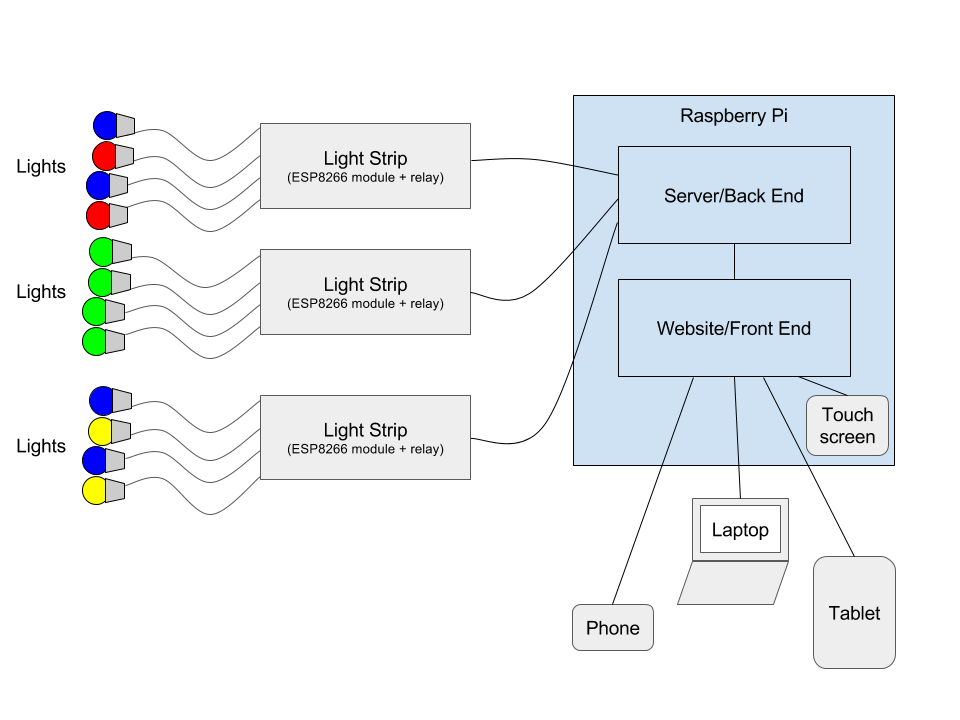
\includegraphics[width=1.0\textwidth]{block-diagram.png}
   \caption{A block-diagram of the structure of PiLight}
\end{figure}
As the diagram shows, the lights are connected to the back end of the server through the ESP devices. These devices are configured to wirelessly connect to the server and receive commands to turn the lights on or off. Each ESP device connects to a relay which can serve up to four different lights. The server then hosts a website that is used to control the lights and the schedules. This website can be viewed by any device that is able to connect to a Wi-Fi network, such as a laptop, smartphone, or tablet. It is also viewable from the touchscreen on the Pi itself.
\subsection{Theory of Operation}
PiLight should provide a way to more easily manage the lights in your home and provide an easy way to schedule times for them to turn on and off. 
